%% Document template source: LaTeX2e template for FEUP's Project FE-UP
%% Document template author: jlopes@fe.up.pt
%% Template adapted

%% A alterar: <--ALTERAR-->

\documentclass[11pt,a4paper]{report}

%% Macros ----------------------------------------------------------------------
\newcommand{\school}{Instituto Superior de Engenharia de Lisboa}
\newcommand{\degree}{Licenciatura em Engenharia Eletrotécnica, Telecomunicações e Computadores}
\newcommand{\projisel}{Projeto ISEL 2023/24 --- LEETC}
\newcommand{\projtitle}{Computer Networks}
\newcommand{\projsubtitle}{Phase 3 - Connecting Multiple Networks}
\newcommand{\projteam}{Grupo LP-07}

%% Package ---------------------------------------------------------------------
\usepackage[a4paper,left=25mm,right=25mm,top=25mm,bottom=25mm,headheight=6mm,footskip=12mm]{geometry}   % Document dimensions
\usepackage[T1]{fontenc}            % PS fonts
\usepackage[english]{babel}         % [portuges]??
\usepackage[export]{adjustbox}      %
\usepackage[normalem]{ulem}         % various types of underlining
\usepackage[table,xcdraw]{xcolor}   % driver-independent color extensions
\usepackage[utf8]{inputenc}         % accents
\usepackage{amsmath}                % multi-line and other mathematical statements
\usepackage{array}                  % Images in tables
\usepackage{booktabs}               %
\usepackage{caption}                % rotating captions, sideways captions, etc.
\usepackage{chicago}                % Bibliography style
\usepackage{color}                  %
\usepackage{fancyhdr}               % Headers and footers
\usepackage{float}                  % tables and figures in the multi-column environment 
\usepackage{graphicx}               % 
\usepackage{hyperref}               % Hyper references
\usepackage{lastpage}               % 
\usepackage{lipsum}                 % loren dummy text
\usepackage{listings}               % Programming syntax
\usepackage{longtable}              % Tables continue in the next page
\usepackage{multicol}               % 
\usepackage{multirow}               % tabular cells spanning multiple rows
\usepackage{newtxtext,newtxmath}    % do not use CM fonts
\usepackage{paralist}
\usepackage{setspace}               % setting the spacing between lines
\usepackage{subcaption}             % for subfigures and the like

%% Package settings ------------------------------------------------------------
\graphicspath{{./images}}                           % {graphicx} - Images path % BY PHASE!!!
\selectlanguage{english}                            % {babel} - Language portuguese
\setlength{\columnsep}{3cm}                         % {multicol} - Column spacement
\definecolor{engineering}{rgb}{0.549,0.176,0.098}   % {color}
\definecolor{cloudwhite}{cmyk}{0,0,0,0.025}         % {color}
\definecolor{deepblue}{rgb}{0,0,0.5}                % {color}
\definecolor{deepred}{rgb}{0.6,0,0}                 % {color}
\definecolor{deepgreen}{rgb}{0,0.5,0}               % {color}
\setlength{\parindent}{0em}                         % {geometry}
\setlength{\parskip}{1ex}                           % {geometry}
\lstdefinestyle{pythoncode}                         % {listings} - Python syntax
{
    aboveskip=8mm,
    backgroundcolor=\color{cloudwhite},             
    basicstyle=\footnotesize\ttfamily,
    numbers=left,                                   % where to put the line-numbers
    belowskip=4mm,
    breakatwhitespace=false,                        % sets if automatic breaks should only happen at whitespace
    breaklines=true,                                % sets automatic line breaking
    captionpos=b,                                   % sets the caption-position to bottom
    escapeinside={\%*}{*)},                         % if you want to add a comment within your code
    float=htb,
    frame=tb,
    keepspaces=true,
    keywordstyle=\bfseries\color{deepblue},
    morekeywords={*,var,template,new}               % if you want to add more keywords to the set
    numbersep=8pt,                                  % how far the line-numbers are from the code
    numberstyle=\scriptsize\texttt,                 % the size of the fonts that are used for the line-numbers
    showspaces=false,                               % show spaces adding particular underscores
    showstringspaces=false,                         % underline spaces within strings
    showtabs=false,                                 % show tabs within strings adding particular underscores
    stepnumber=1,                                   % the step between two line-numbers. If it's 1 each line will be numbered
    stringstyle=\color{deepgreen},
    tabsize=2,                                      % sets default tabsize to 2 spaces
}
\lstdefinestyle{termoutputs}                        % {listings} - Python syntax
{
    aboveskip=8mm,
    backgroundcolor=\color{cloudwhite},             
    basicstyle=\scriptsize\ttfamily,
    numbers=left,                                   % where to put the line-numbers
    belowskip=4mm,
    breakatwhitespace=false,                        % sets if automatic breaks should only happen at whitespace
    breaklines=true,                                % sets automatic line breaking
    captionpos=b,                                   % sets the caption-position to bottom
    escapeinside={\%*}{*)},                         % if you want to add a comment within your code
    float=htb,
    frame=tb,
    keepspaces=true,
    keywordstyle=\bfseries\color{deepblue},
    morekeywords={*,var,template,new}               % if you want to add more keywords to the set
    numbersep=8pt,                                  % how far the line-numbers are from the code
    numberstyle=\scriptsize\texttt,                 % the size of the fonts that are used for the line-numbers
    showspaces=false,                               % show spaces adding particular underscores
    showstringspaces=false,                         % underline spaces within strings
    showtabs=false,                                 % show tabs within strings adding particular underscores
    stepnumber=1,                                   % the step between two line-numbers. If it's 1 each line will be numbered
    stringstyle=\color{deepgreen},
    tabsize=2,                                      % sets default tabsize to 2 spaces
}
\fancyhf{}                                          % {fancyhdr} clear off all default fancyhdr headers and footers
\lfoot{\small{\emph{\projtitle, \projsubtitle}}}    % {fancyhdr}
\rfoot{\small{\thepage\ / \pageref{LastPage}}}      % {fancyhdr}
\pagestyle{fancy}                                   % {fancyhdr} apply the fancy header style
\renewcommand{\headrulewidth}{0.0pt}                % {fancyhdr} no head rule
\renewcommand{\footrulewidth}{0.4pt}                % {fancyhdr}
\hypersetup{                                        % {hyperref}
    plainpages=false,
    pdfpagelayout=SinglePage,
    bookmarksopen=false,
    bookmarksnumbered=true,
    breaklinks=true,
    linktocpage,
    colorlinks=true,
    linkcolor=engineering,
    urlcolor=engineering,
    filecolor=engineering,
    citecolor=engineering,
    allcolors=engineering
}

%% Document start --------------------------------------------------------------
\begin{document}
    \pagenumbering{roman}\setcounter{page}{1}

%% Cover -----------------------------------------------------------------------
\begin{titlepage}
    \center

    \vspace*{-12mm}
    {\large \textbf{\textsc{\school}}}\\

    \vfill

    
\includegraphics[width=62mm]{logoisel}
    
    \vfill
    
    {\huge \textbf{\projtitle}}\\[6mm]
    {\Large \textbf{\projsubtitle}}\\
    
    \vfill
    
    \vfill
    
    {\Large \textbf{\projisel}}\\[12mm]
    
    {\Large \textbf{Coordination}}\\[4mm]
    {\large General: Carlos Meneses\hspace*{18mm}
            Course: Nuno Cruz}\\[6mm]
    
    {\Large \textbf{\projteam}}\\[4mm]
    {\large Supervisor: Luís Pires\hspace*{12mm}}\\[6mm]
    
    {\Large \textbf{Student}}\\[4mm]
    {\large Nuno Brito $<$A46948@alunos.isel.pt$>$}
    
    \vspace*{10mm}
    
    \renewcommand{\today}{May 19th 2024}
    \today
    
\end{titlepage}

%% TOC -------------------------------------------------------------------------
\tableofcontents

%% List of figures -------------------------------------------------------------
\listoffigures
\addcontentsline{toc}{chapter}{Figure list}

%% List of tables --------------------------------------------------------------
\listoftables
\addcontentsline{toc}{chapter}{Table list}

%% List of listings --------------------------------------------------------------
\lstlistoflistings
\addcontentsline{toc}{chapter}{Listings list}

%% Acronyms --------------------------------------------------------------------
\chapter*{Acronyms list}
    \addcontentsline{toc}{chapter}{Acronyms list}

    \begin{flushleft}
        \begin{tabular}{l p{0.8\linewidth}}
            API     & Application Programming Interface\\
            CLI     & Command Line Interface\\
            CMD     & Command Prompt\\
            GUI     & Graphical User Interface\\
            HTTP    & Hyper Text Transfer Protocol\\
            HTTPS   & Hyper Text Transfer Protocol Secure\\
            IP      & Internet Protocol\\
            IPv4    & Internet Protocol version 4\\
            IPv6    & Internet Protocol version 6\\
            LAN     & Local Area Network\\
            OS      & Operating System\\
            OSS     & openSUSE\\
            PC      & Personal Computer\\
            PHP     & PHP: Hypertext Preprocessor\\
            SSL     & Secure Sockets Layer\\
            TCP     & Transmission Control Protocol\\
            TLS     & Transport Layer Security\\
            TUI     & Terminal User Interface\\ % Not used yet
            UDP     & User Datagram Protocol\\
            VPN     & Virtual Private Network\\
            WWW     & World Wide Web\\
            XAMPP   & Cross-Platform, Apache, MySQL, PHP, and Perl
        \end{tabular}
    \end{flushleft}

%% Glossary --------------------------------------------------------------------
\chapter*{Glossary}
    \addcontentsline{toc}{chapter}{Glossary}

    \begin{description}
        \item[Apache2] \hfill \\
            An opensource HTTP web server.
        \item[Bit] \hfill \\
            A unit of information in computing and digital communications. The bit represents a logical state with one of two possible values, 0 or 1 (other representations such as \textit{true / false} are also valid).
        \item[Byte] \hfill \\
            Also a unit of digital information, consists of 8 bits.
        \item[Broadcast] \hfill \\
            A method of transferring a message to all recipients simultaneously.
        \item[Browser] \hfill \\
            A browser is a internet navigation software. It comes in multiple flavours, nowadays the big three are Microsoft Edge, Mozilla Firefox and Google Chrome.
        \item[Cisco Packet Tracer] \hfill \\
            A cross-platform visual network simulation tool.
        \item[Command Prompt] \hfill \\
            The default command-line interpreter for Windows operating systems.
        \item[Firewall] \hfill \\
            A barrier between networks. Controls inbound and outbound traffic.
        \item[Gateway] \hfill \\
            A network gateway provides a connection between networks and devices. Known as protocol translation gateways or mapping gateways, can perform protocol conversions to connect networks with different network protocol technologies.
        \item[LibreWolf] \hfill \\
            An internet browser based on Mozilla's Firefox. It's primary purpose is to allow privacy, and with it comes security. It achieves this by removing telemetry and data collection.
        \item[Linux] \hfill \\
            Open-source Unix-like operating systems based on the Linux kernel.
        \item[MariaDB] \hfill \\
            A community-developed fork of MySQL database server.
        \item[openSUSE Tumbleweed] \hfill \\
            An openSUSE (OSS) is an open-source community driven Linux-based distribuition sponsored by SUSE Software Solutions. Tumbleweed is a rolling release version allowing for up-to-date software releases.
        \item[Operating system] \hfill \\
            A program that manages a computer's resources from software to hardware.
        \item[Ping] \hfill \\
             A software utility used to test the reachability of a host on an IP network.
        \item[Tracert] \hfill \\
            Or \textbf{traceroute} in unix and linux systems, is a computer network diagnostic command for displaying possible routes and measuring transit delays of packets across an IP network.
        \item[Ipconfig] \hfill \\
            Or \textbf{ifconfig} in unix and linux systems, is a console application program that displays all current TCP/IP network configuration values.
        \item[Python] \hfill \\
            Python is a high-level programming language, object-oriented.
        \item[Perl] \hfill \\
            A high-level, general-purpose, interpreted, dynamic programming language
        \item[Rolling release distribuition] \hfill \\
            A distribuition where it's software release cycle is more frequent than those of Long Term Support (LTS). It's up to the Linux-based distribuitor to guarantee the testing of a package.
        \item[Router] \hfill \\
            A networking device that forwards data packets between computer networks, including internetworks such as the global Internet.
        \item[Switch] \hfill \\
            A networking hardware that connects devices on a computer network by using packet switching to receive and forward data to the destination device.
        \item[Socket] \hfill \\
            A network socket serves as an endpoint for sending and receiving data across the network.
        \item[Subnet Mask] \hfill \\
            Is a logical subdivision of an IP network.
        \item[Unix] \hfill \\
            Is a family of multitasking, multi-user computer operating systems that derive from the original AT\&T Unix.
        \item[VPN] \hfill \\
            A private network creating a secure connection between a device and a network.
        \item[Windows] \hfill \\
            Microsoft's operating system. First released in 1985 as a Graphical User Interface (GUI) for MS-DOS, continued to evolve with it's latest version being 11.
            Due to it's nature, it's not recommended for server production environment.
        \item[Wireshark] \hfill \\
            Wireshark is a network protocol analyser software. Allows traffic capture between a computer and a network.
        \item[XAMPP] \hfill \\
            A software package environment collection containing Apache2 webserver, MariaDB database, PHP and Perl.
    \end{description}

%% Chapter: introduction -------------------------------------------------------
\chapter{Introduction}
% display headers & footers
    \pagestyle{fancy}
    For this phase we're going to expand on the previous phase 2 outline. \\
    Conveniently taking advantage of the work already performed, it's time to execute it. If only it were that simple.
    As we'll see, firstly correcting the IP assigments to meet the right standards, then re-applying those new IP addresses to the network.

% main page numbers with arabic numerals
    \pagenumbering{arabic}\setcounter{page}{1}

%% Chapter: phase 3 ------------------------------------------------------------
\chapter{Phase 3}
    Taking information from the previous phase 2 project, this is what we're re-applying:
    \begin{compactitem}
        \item IP range: 192.168.\textbf{\textit{GROUP NUMBER}}.0.
        \item Commands:
        \begin{compactitem}
            \item ping: to test connectivity between devices over IP.
            \item tracert: diagnostic command for displaying possible routes, also measures transit delay of packages across IP.
            \item ipconfig: console application program of some computer operating systems that displays all current TCP/IP network configuration values. Unix and linux equivalent is \textit{ifconfig}.
        \end{compactitem}
    \end{compactitem}

    Now for the specific requirements in phase 3. Most of it was already accomplished in phase 2.
    The mathemathical formula is still valid here:\\
    \[
        Clients_{LAN_A} = max\left(20, \left(\sum_{k=0}^n studentnumber_k\right)mod 100\right)\quad <=> 
        Clients_{LAN_A} = 48\quad
    \] \\
    \[
        Clients_{LAN_B} = \frac{Clients_{LAN_A}}{2}\quad <=>
        Clients_{LAN_B} = 27\quad
    \]\\

    What about our network diagram? Well, it's still pretty much the same with only one small caveat, static routes.\\
    This circuit must obey the subsequent rules:
    \begin{compactitem}
        \item Connection between LAN's A and B to LAN Servers always go through router R1 to router R2.
        \item LAN's A and B with outside destination always use the router R1 and router R0 path.
        \item LAN server to the outside must go through router R2 and router R0.
    \end{compactitem}

    \begin{figure}[h]
        \centering
        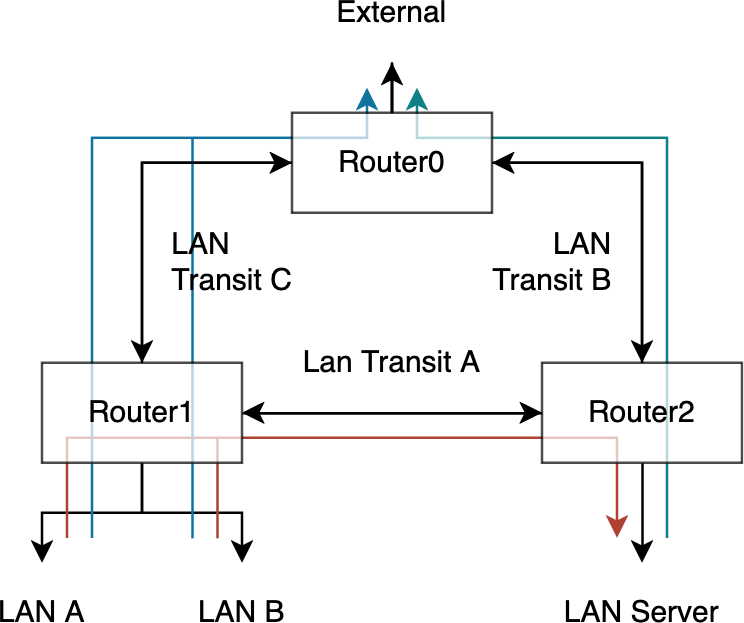
\includegraphics[scale=0.40,valign=c]{diagramL250}
        \caption{Phase 3 simplified network diagram}
        \label{fig:p2netdiag}
    \end{figure}

    \pagebreak

    \begin{longtable}[c]{@{}lllllclc@{}}
        \toprule
        \textbf{Router}     & \textbf{From}                  & \textbf{To} & \textbf{Network} & \textbf{Via}                                       & \multicolumn{3}{c}{\textbf{Through}}                                        \\* \midrule
        \endfirsthead
        %
        \multicolumn{8}{c}%
        {{\bfseries Table \thetable\ continued from previous page}} \\
        \toprule
        \textbf{Router}     & \textbf{From}                  & \textbf{To} & \textbf{Network} & \textbf{Via}                                       & \multicolumn{3}{c}{\textbf{Through}}                                        \\* \midrule
        \endhead
        %
        \multirow{2}{*}{R1} & \multirow{2}{*}{LAN A / LAN B} & LAN Servers & 192.168.7.0/25   & 192.168.7.254                                      & \multirow{2}{*}{R1} & \textgreater{}                  & R2                  \\
                            &                                & Any         & 8.8.8.8/30       & 192.168.7.249                                      &                     & \textgreater{}                  & R0                  \\* \midrule
        \multirow{3}{*}{R2} & \multirow{3}{*}{LAN Servers}   & LAN A       & 192.168.7.128/26 & \multicolumn{1}{c}{\multirow{2}{*}{192.168.7.253}} & \multirow{3}{*}{R2} & \multirow{2}{*}{\textgreater{}} & \multirow{2}{*}{R1} \\
                            &                                & LAN B       & 192.168.7.192/27 & \multicolumn{1}{c}{}                               &                     &                                 &                     \\* \cmidrule(lr){3-5} \cmidrule(l){7-8}
                            &                                & Any         & 8.8.8.8/30       & 192.168.7.245                                      &                     & \textgreater{}                  & R0                  \\* \midrule
        \multirow{3}{*}{R0} & \multirow{3}{*}{Any}           & LAN A       & 192.168.7.128/26 & \multicolumn{1}{c}{\multirow{2}{*}{192.168.7.250}} & \multirow{3}{*}{R0} & \multirow{2}{*}{\textgreater{}} & \multirow{2}{*}{R1} \\
                            &                                & LAN B       & 192.168.7.192/27 & \multicolumn{1}{c}{}                               &                     &                                 &                     \\* \cmidrule(lr){3-5} \cmidrule(l){7-8}
                            &                                & LAN Servers & 192.168.7.0/25   & 192.168.7.246                                      &                     & \textgreater{}                  & R2                  \\* \bottomrule
        \caption{Static routes table}
        \label{tab:staticroutetbl}\\
    \end{longtable}
    
    \section{Outline}
        Previously the subdivision was perfomed by opening with the lowest subdivision, \textbf{/30}, then expanding till \textbf{/25}. \\
        However, this was inappropriate due to best practices rules which assert that network subdivision starts with the largest network, \textbf{/25}, and then continues till the smallest network, \textbf{/30}. \\

        And so, here are the results:
        \begin{longtable}[c]{rcccccccccccccccc}
            \hline
            \multicolumn{1}{c}{}                                                                       & \multicolumn{16}{c}{\textbf{IP}}                                                                                                                                                                                                                                                                                                                                                                                                                                                                                  \\
            \multicolumn{1}{c}{\multirow{-2}{*}{\textbf{Subnet}}}                                      & \cellcolor[HTML]{F4B084}0     & \cellcolor[HTML]{F4B084}127    & \cellcolor[HTML]{A9D08E}128    & \cellcolor[HTML]{A9D08E}191   & \cellcolor[HTML]{FFD966}192    & \cellcolor[HTML]{FFD966}223   & \cellcolor[HTML]{BFBFBF}224    & \cellcolor[HTML]{BFBFBF}239   & \cellcolor[HTML]{C09FE5}240 & \cellcolor[HTML]{C09FE5}243 & \cellcolor[HTML]{C09FE5}244 & \cellcolor[HTML]{C09FE5}247 & \cellcolor[HTML]{C09FE5}248 & \cellcolor[HTML]{C09FE5}251 & \cellcolor[HTML]{C09FE5}252 & \cellcolor[HTML]{C09FE5}255 \\ \hline
            \endfirsthead
            %
            \multicolumn{17}{c}%
            {{\bfseries Table \thetable\ continued from previous page}} \\
            \hline
            \multicolumn{1}{c}{}                                                                       & \multicolumn{16}{c}{\textbf{IP}}                                                                                                                                                                                                                                                                                                                                                                                                                                                                                  \\
            \multicolumn{1}{c}{\multirow{-2}{*}{\textbf{Subnet}}}                                      & \cellcolor[HTML]{F4B084}0     & \cellcolor[HTML]{F4B084}127    & \cellcolor[HTML]{A9D08E}128    & \cellcolor[HTML]{A9D08E}191   & \cellcolor[HTML]{FFD966}192    & \cellcolor[HTML]{FFD966}223   & \cellcolor[HTML]{BFBFBF}224    & \cellcolor[HTML]{BFBFBF}239   & \cellcolor[HTML]{C09FE5}240 & \cellcolor[HTML]{C09FE5}243 & \cellcolor[HTML]{C09FE5}244 & \cellcolor[HTML]{C09FE5}247 & \cellcolor[HTML]{C09FE5}248 & \cellcolor[HTML]{C09FE5}251 & \cellcolor[HTML]{C09FE5}252 & \cellcolor[HTML]{C09FE5}255 \\ \hline
            \endhead
            %
            \hline
            \endfoot
            %
            \endlastfoot
            %
            \textbf{/30}                                                                               &                               &                                &                                &                               &                                &                               &                                &                               &                             &                             &                             &                             &                             &                             & \cellcolor[HTML]{C09FE5}    & \cellcolor[HTML]{C09FE5}    \\
            \textbf{/30}                                                                               &                               &                                &                                &                               &                                &                               &                                &                               &                             &                             &                             &                             & \cellcolor[HTML]{C09FE5}    & \cellcolor[HTML]{C09FE5}    &                             &                             \\
            \textbf{/30}                                                                               &                               &                                &                                &                               &                                &                               &                                &                               &                             &                             & \cellcolor[HTML]{C09FE5}    & \cellcolor[HTML]{C09FE5}    &                             &                             &                             &                             \\
            \textbf{/30}                                                                               &                               &                                &                                &                               &                                &                               &                                &                               & \cellcolor[HTML]{C09FE5}    & \cellcolor[HTML]{C09FE5}    &                             &                             &                             &                             &                             &                             \\
            \textbf{/28}                                                                               &                               &                                &                                &                               &                                &                               & \cellcolor[HTML]{BFBFBF}       & \cellcolor[HTML]{BFBFBF}      &                             &                             &                             &                             &                             &                             &                             &                             \\
            \textbf{/27}                                                                               &                               &                                &                                &                               & \cellcolor[HTML]{FFD966}       & \cellcolor[HTML]{FFD966}      &                                &                               &                             &                             &                             &                             &                             &                             &                             &                             \\
            \textbf{/26}                                                                               &                               &                                & \cellcolor[HTML]{A9D08E}       & \cellcolor[HTML]{A9D08E}      &                                &                               &                                &                               &                             &                             &                             &                             &                             &                             &                             &                             \\
            \textbf{/25}                                                                               & \cellcolor[HTML]{F4B084}      & \cellcolor[HTML]{F4B084}       &                                &                               &                                &                               &                                &                               &                             &                             &                             &                             &                             &                             &                             &                             \\ \hline
                                                                                                       & \multicolumn{16}{r}{\cellcolor[HTML]{00B0F0}/24}                                                                                                                                                                                                                                                                                                                                                                                                                                                                  \\
                                                                                                       & \multicolumn{2}{r}{\cellcolor[HTML]{F4B084}}                   & \multicolumn{14}{r}{\cellcolor[HTML]{F4B084}/25}                                                                                                                                                                                                                                                                                                                                                                                                 \\
                                                                                                       & \multicolumn{2}{r}{\cellcolor[HTML]{F4B084}}                   & \multicolumn{2}{r}{\cellcolor[HTML]{A9D08E}}                   & \multicolumn{12}{r}{\cellcolor[HTML]{A9D08E}/26}                                                                                                                                                                                                                                                                                                                                \\
                                                                                                       & \multicolumn{2}{r}{\cellcolor[HTML]{F4B084}}                   & \multicolumn{2}{r}{\cellcolor[HTML]{A9D08E}}                   & \multicolumn{2}{r}{\cellcolor[HTML]{FFD966}}                   & \multicolumn{10}{r}{\cellcolor[HTML]{FFD966}/27}                                                                                                                                                                                                                                                               \\
                                                                                                       & \multicolumn{2}{r}{\cellcolor[HTML]{F4B084}}                   & \multicolumn{2}{r}{\cellcolor[HTML]{A9D08E}}                   & \multicolumn{2}{r}{\cellcolor[HTML]{FFD966}}                   & \multicolumn{2}{r}{\cellcolor[HTML]{BFBFBF}}                   & \multicolumn{8}{r}{\cellcolor[HTML]{BFBFBF}/28}                                                                                                                                                                                               \\
                                                                                                       & \multicolumn{2}{r}{\multirow{-5}{*}{\cellcolor[HTML]{F4B084}}} & \multicolumn{2}{r}{\multirow{-4}{*}{\cellcolor[HTML]{A9D08E}}} & \multicolumn{2}{r}{\multirow{-3}{*}{\cellcolor[HTML]{FFD966}}} & \multicolumn{2}{r}{\multirow{-2}{*}{\cellcolor[HTML]{BFBFBF}}} & \multicolumn{4}{r}{/29}                                                                                               & \multicolumn{4}{r}{/29}                                                                                               \\
            \multirow{-7}{*}{\textbf{\begin{tabular}[c]{@{}r@{}}Subnet\\ visual\\ split\end{tabular}}} & \multicolumn{2}{r}{\cellcolor[HTML]{F4B084}/25}                & \multicolumn{2}{r}{\cellcolor[HTML]{A9D08E}/26}                & \multicolumn{2}{r}{\cellcolor[HTML]{FFD966}/27}                & \multicolumn{2}{r}{\cellcolor[HTML]{BFBFBF}/28}                & \multicolumn{2}{r}{\cellcolor[HTML]{C09FE5}/30}           & \multicolumn{2}{r}{\cellcolor[HTML]{C09FE5}/30}           & \multicolumn{2}{r}{\cellcolor[HTML]{C09FE5}/30}           & \multicolumn{2}{r}{\cellcolor[HTML]{C09FE5}/30}           \\ \hline
            \caption{Visual LAN allocation}
            \label{tab:visuallanalloc}\\
        \end{longtable}

        \begin{longtable}[c]{lllllll}
            \hline
                                                                                                  & \textbf{Network}            & \textbf{Usable IPs} & \textbf{Router} & \textbf{Broadcast} & \multicolumn{1}{c}{\textbf{Subnet Mask}} &                                      \\ \cline{2-5}
            \multirow{-2}{*}{\textbf{Name}}                                                       & \multicolumn{4}{c}{192.168.7.}                                                           & \multicolumn{1}{c}{255.255.255.}         & \multirow{-2}{*}{\textbf{Populated}} \\ \hline
            \endfirsthead
            %
            \multicolumn{7}{c}%
            {{\bfseries Table \thetable\ continued from previous page}} \\
            \hline
                                                                                                  & \textbf{Network}            & \textbf{Usable IPs} & \textbf{Router} & \textbf{Broadcast} & \multicolumn{1}{c}{\textbf{Subnet Mask}} &                                      \\ \cline{2-5}
            \multirow{-2}{*}{\textbf{Name}}                                                       & \multicolumn{4}{c}{192.168.7.}                                                           & \multicolumn{1}{c}{255.255.255.}         & \multirow{-2}{*}{\textbf{Populated}} \\ \hline
            \endhead
            %
            \hline
            \endfoot
            %
            \endlastfoot
            %
            \cellcolor[HTML]{F4B084}\textbf{LAN Server}                                           & 0                           & 1 - 125             & 126             & 127                & 128                                      & 126                                  \\
            \cellcolor[HTML]{A9D08E}\textbf{LAN A}                                                & 128                         & 129 - 189           & 190             & 191                & 192                                      & 48                                   \\
            \cellcolor[HTML]{FFD966}\textbf{LAN B}                                                & 192                         & 193 - 221           & 222             & 223                & 224                                      & 27                                   \\ \hline
            \multirow{+2}{*}{\textbf{\begin{tabular}[c]{@{}l@{}}Unused\\ remaining\end{tabular}}} & \cellcolor[HTML]{BFBFBF}224 & 225 - 238           &                 & 239                &                                          & 0                                    \\
                                                                                                  & \cellcolor[HTML]{C09FE5}240 & 241 - 242           &                 & 243                &                                          & 0                                    \\ \hline
            \cellcolor[HTML]{C09FE5}\textbf{LAN Transit C}                                        & 244                         & 245 - 246           &                 & 247                & 252                                      & 2                                    \\
            \cellcolor[HTML]{C09FE5}\textbf{LAN Transit B}                                        & 248                         & 249 - 250           &                 & 251                & 252                                      & 2                                    \\
            \cellcolor[HTML]{C09FE5}\textbf{LAN Transit A}                                        & 252                         & 253 - 254           &                 & 255                & 252                                      & 2                                    \\ \hline
            \caption{LAN allocation table}
            \label{tab:lanalloctable}\\
        \end{longtable}

        \begin{longtable}[c]{@{}llrllrr@{}}
            \toprule
            \multicolumn{1}{c}{\multirow{3}{*}{\textbf{Name}}} & \multicolumn{2}{c}{\multirow{2}{*}{\textbf{Ports Link}}} & \multicolumn{1}{c}{\multirow{3}{*}{\textbf{Network}}} & \multicolumn{1}{c}{\multirow{2}{*}{\textbf{IP}}} & \multicolumn{1}{c}{\multirow{2}{*}{\textbf{Gateway}}} & \multicolumn{1}{c}{\multirow{2}{*}{\textbf{Subnet Mask}}} \\
            \multicolumn{1}{c}{}                               & \multicolumn{2}{c}{}                                     & \multicolumn{1}{c}{}                                  & \multicolumn{1}{c}{}                             & \multicolumn{1}{c}{}                                  & \multicolumn{1}{c}{}                                      \\* \cmidrule(lr){2-3} \cmidrule(l){5-7}
            \multicolumn{1}{c}{}                               & \textbf{From}                & \textbf{To}               & \multicolumn{1}{c}{}                                  & \multicolumn{2}{c}{192.168.7.}                                                                           & \multicolumn{1}{c}{255.255.255.}                          \\* \midrule
            \endfirsthead
            %
            \multicolumn{7}{c}%
            {{\bfseries Table \thetable\ continued from previous page}} \\
            \toprule
            \multicolumn{1}{c}{\multirow{3}{*}{\textbf{Name}}} & \multicolumn{2}{c}{\multirow{2}{*}{\textbf{Ports Link}}} & \multicolumn{1}{c}{\multirow{3}{*}{\textbf{Network}}} & \multicolumn{1}{c}{\multirow{2}{*}{\textbf{IP}}} & \multicolumn{1}{c}{\multirow{2}{*}{\textbf{Gateway}}} & \multicolumn{1}{c}{\multirow{2}{*}{\textbf{Subnet Mask}}} \\
            \multicolumn{1}{c}{}                               & \multicolumn{2}{c}{}                                     & \multicolumn{1}{c}{}                                  & \multicolumn{1}{c}{}                             & \multicolumn{1}{c}{}                                  & \multicolumn{1}{c}{}                                      \\* \cmidrule(lr){2-3} \cmidrule(l){5-7}
            \multicolumn{1}{c}{}                               & \textbf{From}                & \textbf{To}               & \multicolumn{1}{c}{}                                  & \multicolumn{2}{c}{192.168.7.}                                                                           & \multicolumn{1}{c}{255.255.255.}                          \\* \midrule
            \endhead
            %
            \bottomrule
            \endfoot
            %
            \endlastfoot
            %
            \textbf{PC0}                                       & Fa0                          & Sw0 Fa0/2                 & \multirow{2}{*}{LAN A}                                & 129                                              & \multirow{2}{*}{190}                                  & \multirow{2}{*}{192}                                      \\
            \textbf{Laptop0}                                   & Fa0                          & Sw0 Fa0/3                 &                                                       & 130                                              &                                                       &                                                           \\* \midrule
            \textbf{PC1}                                       & Fa0                          & Sw1 Fa0/2                 & \multirow{2}{*}{LAN B}                                & 193                                              & \multirow{2}{*}{222}                                  & \multirow{2}{*}{224}                                      \\
            \textbf{Laptop1}                                   & Fa0                          & Sw1 Fa0/3                 &                                                       & 194                                              &                                                       &                                                           \\* \midrule
            \multirow{3}{*}{\textbf{R0}}                       & Fa0/0                        & Fa0/0                     & External                                              &                                                  &                                                       & \multicolumn{1}{l}{}                                      \\* \cmidrule(l){5-7}
                                                               & Fa4/0                        & R2 Fa4/0                  & LAN Transit C                                         & 245                                              &                                                       & \multirow{2}{*}{252}                                      \\
                                                               & Fa5/0                        & R1 Fa5/0                  & LAN Transit B                                         & 249                                              &                                                       &                                                           \\* \midrule
            \multirow{4}{*}{\textbf{R1}}                       & Fa0/0                        & Sw0 Fa0/1                 & LAN A                                                 & 190                                              &                                                       & \multicolumn{1}{l}{192}                                   \\
                                                               & Fa1/0                        & Sw1 Fa0/1                 & LAN B                                                 & 222                                              &                                                       & \multicolumn{1}{l}{224}                                   \\* \cmidrule(l){5-7}
                                                               & Fa4/0                        & R2 Fa5/0                  & LAN Transit A                                         & 253                                              &                                                       & \multirow{2}{*}{252}                                      \\
                                                               & Fa5/0                        & R1 Fa4/0                  & LAN Transit B                                         & 250                                              &                                                       &                                                           \\* \midrule
            \multirow{3}{*}{\textbf{R2}}                       & Fa0/0                        & Sw2 Fa0/4                 & LAN Server                                            & 126                                              &                                                       & \multicolumn{1}{l}{128}                                   \\* \cmidrule(l){5-7}
                                                               & Fa4/0                        & R0 Fa4/0                  & LAN Transit C                                         & 246                                              &                                                       & \multirow{2}{*}{252}                                      \\
                                                               & Fa5/0                        & R1 Fa4/0                  & LAN Transit A                                         & 254                                              &                                                       &                                                           \\* \midrule
            \textbf{HTTP-Server}                               & Fa0                          & Sw2 Fa0/1                 & \multirow{3}{*}{LAN Server}                           & 3                                                & \multirow{3}{*}{126}                                  & \multirow{3}{*}{128}                                      \\
            \textbf{DNS-Server}                                & Fa0                          & Sw2 Fa0/2                 &                                                       & 2                                                &                                                       &                                                           \\
            \textbf{DHCP-Server}                               & Fa0                          & Sw2 Fa0/3                 &                                                       & 1                                                &                                                       &                                                           \\* \midrule
            \multirow{3}{*}{\textbf{Sw0}}                      & Fa0/1                        & R1 Fa0/0                  & \multirow{3}{*}{LAN A}                                & \multicolumn{3}{c}{\multirow{3}{*}{}}                                                                                                                                \\
                                                               & Fa0/2                        & PC0                       &                                                       & \multicolumn{3}{c}{}                                                                                                                                                 \\
                                                               & Fa0/3                        & Laptop0                   &                                                       & \multicolumn{3}{c}{}                                                                                                                                                 \\* \midrule
            \multirow{3}{*}{\textbf{Sw1}}                      & Fa0/1                        & R1 Fa1/0                  & \multirow{3}{*}{LAN B}                                & \multicolumn{3}{c}{\multirow{3}{*}{}}                                                                                                                                \\
                                                               & Fa0/2                        & PC1                       &                                                       & \multicolumn{3}{c}{}                                                                                                                                                 \\
                                                               & Fa0/3                        & Laptop1                   &                                                       & \multicolumn{3}{c}{}                                                                                                                                                 \\* \midrule
            \multirow{4}{*}{\textbf{Sw2}}                      & Fa0/1                        & HTTP-Server               & \multirow{4}{*}{LAN Server}                           & \multicolumn{3}{c}{\multirow{4}{*}{}}                                                                                                                                \\
                                                               & Fa0/2                        & DNS-Server                &                                                       & \multicolumn{3}{c}{}                                                                                                                                                 \\
                                                               & Fa0/3                        & DHCP-Server               &                                                       & \multicolumn{3}{c}{}                                                                                                                                                 \\
                                                               & Fa0/4                        & R2 Fa0/0                  &                                                       & \multicolumn{3}{c}{}                                                                                                                                                 \\* \bottomrule
            \caption{IP configuration table}
            \label{tab:ipconftable}\\
        \end{longtable}

        Beautifully charted. Let's implement it with our favorite tool, Cisco Packet Trace.

    \section{Configuring devices}
        \begin{flushleft}
                \begin{center}
                    \begin{longtable}{ m{5cm} l }
                        \textbf{Steps} & \textbf{Example} \\
                        \hline
                        \endfirsthead
                        \multicolumn{2}{c}%
                        {{\bfseries Table \thetable\ continued from previous page}} \\
                        \textbf{Steps} & \textbf{Example} \\
                        \hline
                        \endhead
                        \hline Continued on next page \\
                        \endfoot
                        \endlastfoot

                        To configure the IP on a device we must \textbf{single-click} in the intended device (1), go to the \textit{desktop tab} (2) and select \textit{IP Configuration} (3).  & 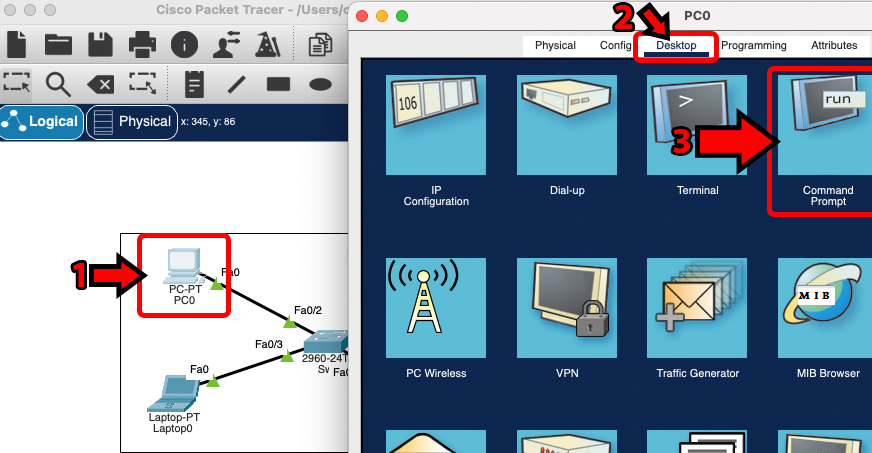
\includegraphics[scale=0.32 ,valign=c]{CiscoPacketTracer_cmdOutput}   \\ \hline
                        IP configuration for LAN A, PC0 and Laptop0.                                                                                                                            & 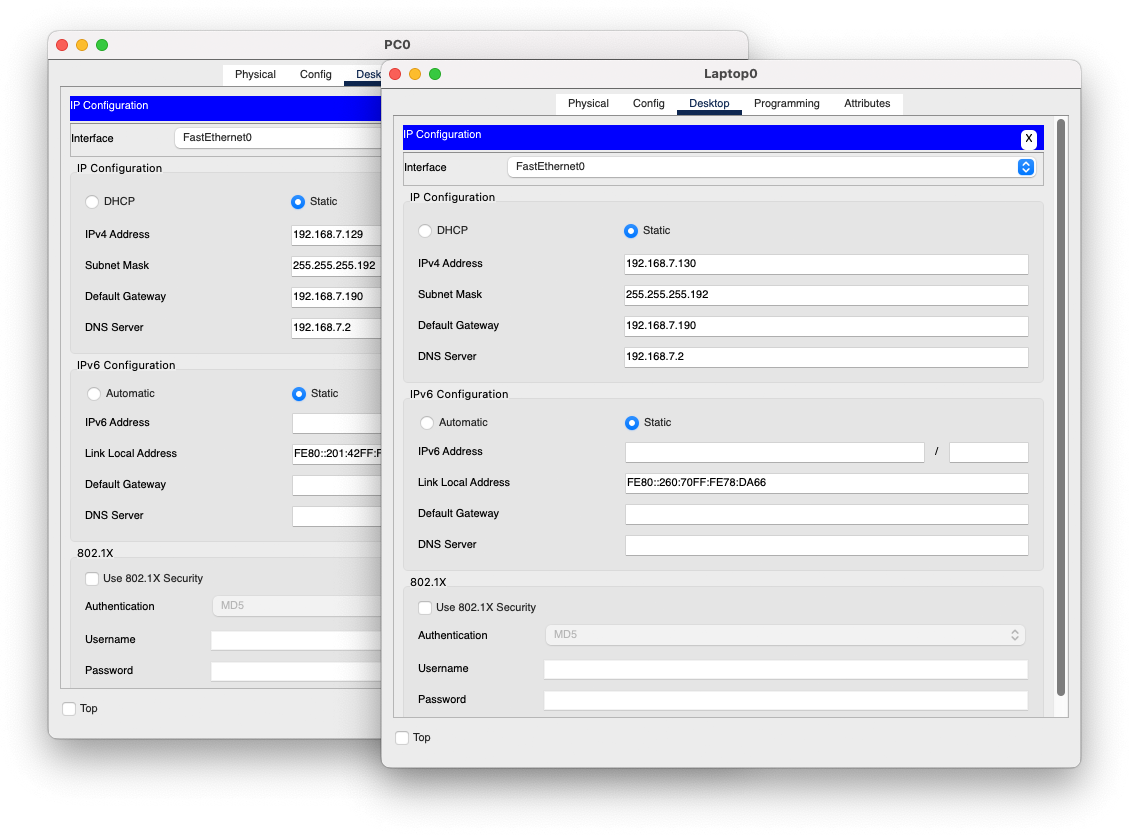
\includegraphics[scale=0.25 ,valign=c]{lana-ipall}                    \\ \hline
                        IP configuration for LAN B, PC1 and Laptop1.                                                                                                                            & 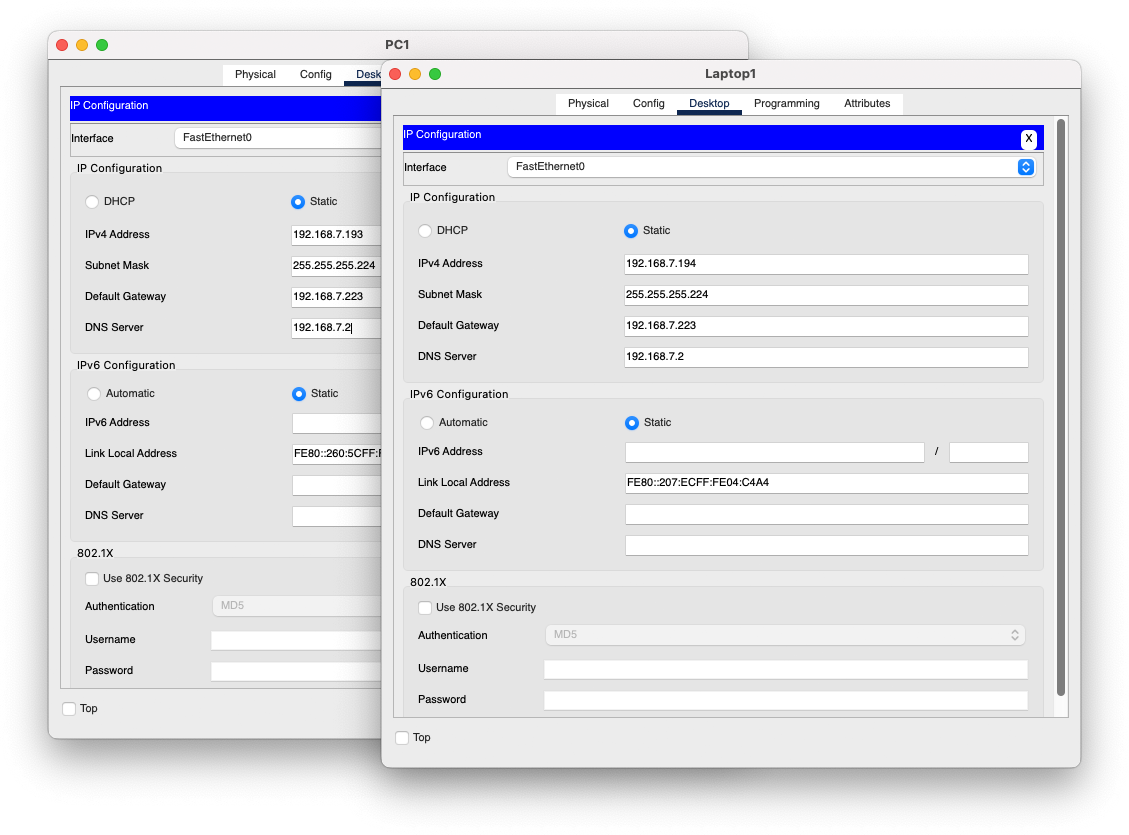
\includegraphics[scale=0.25 ,valign=c]{lanb-ipall}                    \\ \hline
                        IP configuration for LAN Servers, DHCP-Server, DNS-Server and HTTP-Server.                                                                                              & 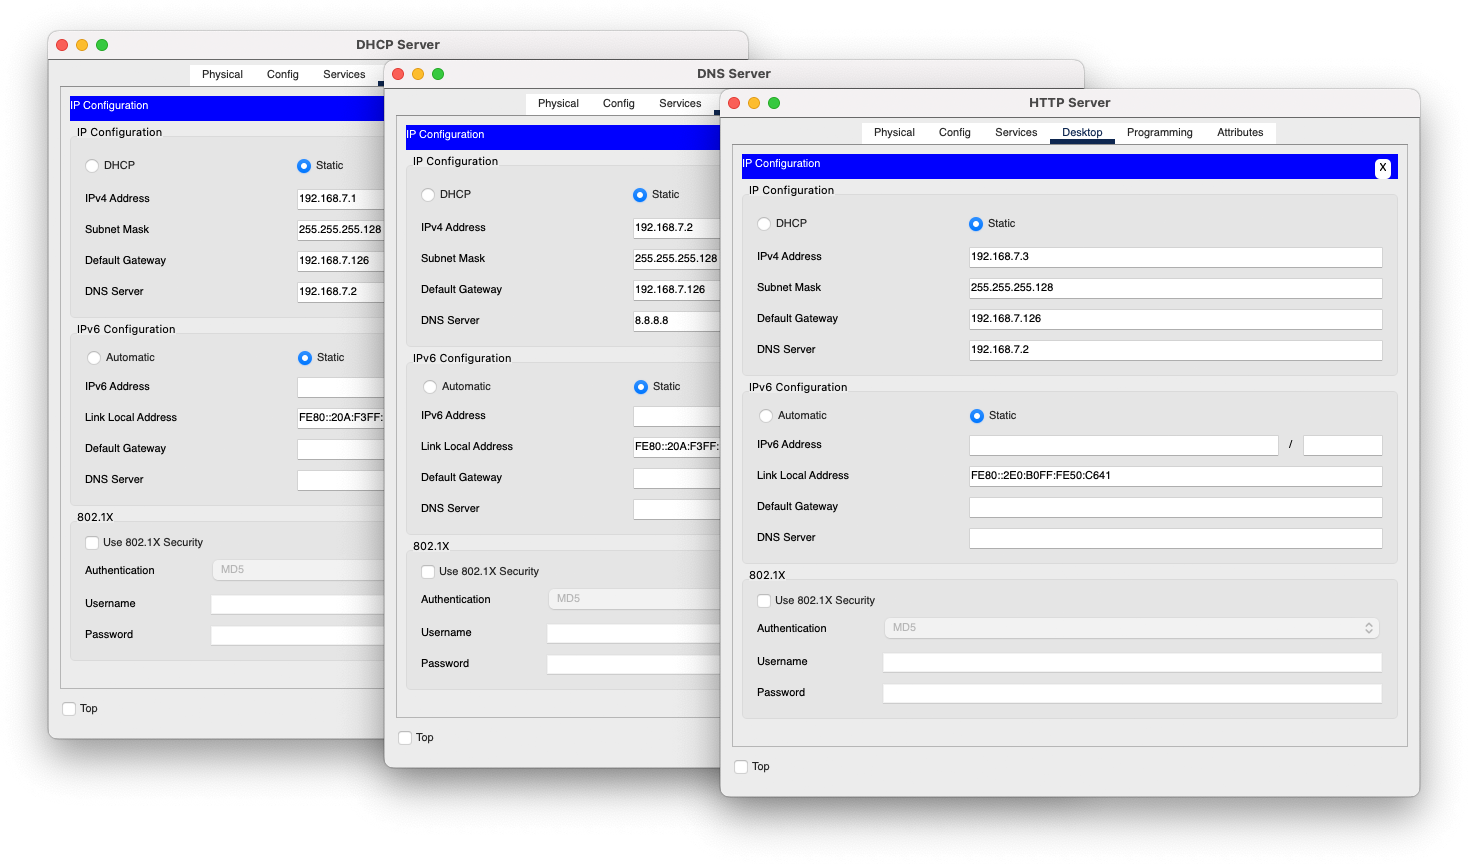
\includegraphics[scale=0.19 ,valign=c]{lanservers-ipall}              \\ \hline

                        \caption{Cisco Packet Tracer IP device guide}
                        \label{tab:cptg1}
                    \end{longtable}
                \end{center}
        \end{flushleft}

    \section{Configuring routers}
        For the router there's two options, both valid and exhibited in the report. The graphical user interface (GUI) in the right and the command line interface (CLI) in the output subsection. Going by the GUI it's crystal clear, just input the necessary IP and subnet mask. And also the static routes.

        \begin{flushleft}
                \begin{center}
                    \begin{longtable}{ m{5cm} l }
                        \textbf{Steps} & \textbf{Example} \\
                        \hline
                        \endfirsthead
                        \multicolumn{2}{c}%
                        {{\bfseries Table \thetable\ continued from previous page}} \\
                        \textbf{Steps} & \textbf{Example} \\
                        \hline
                        \endhead
                        \hline Continued on next page \\
                        \endfoot
                        \endlastfoot

                        IP configuration for Router 0.  & 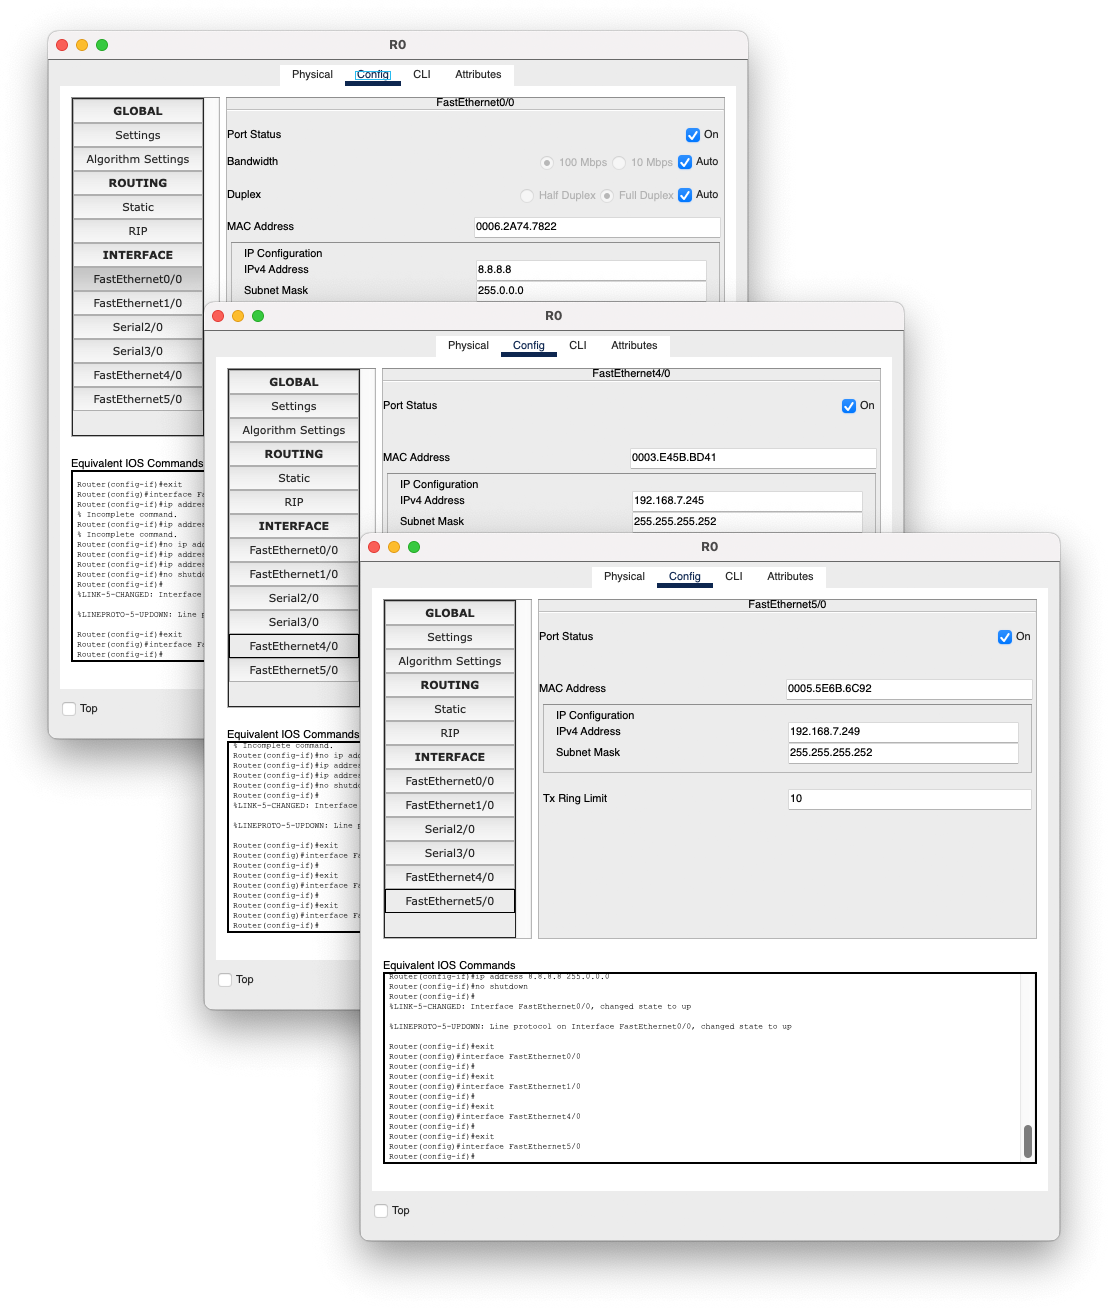
\includegraphics[scale=0.245 ,valign=c]{r0-ipall}                      \\ \hline
                        IP configuration for Router 1.  & 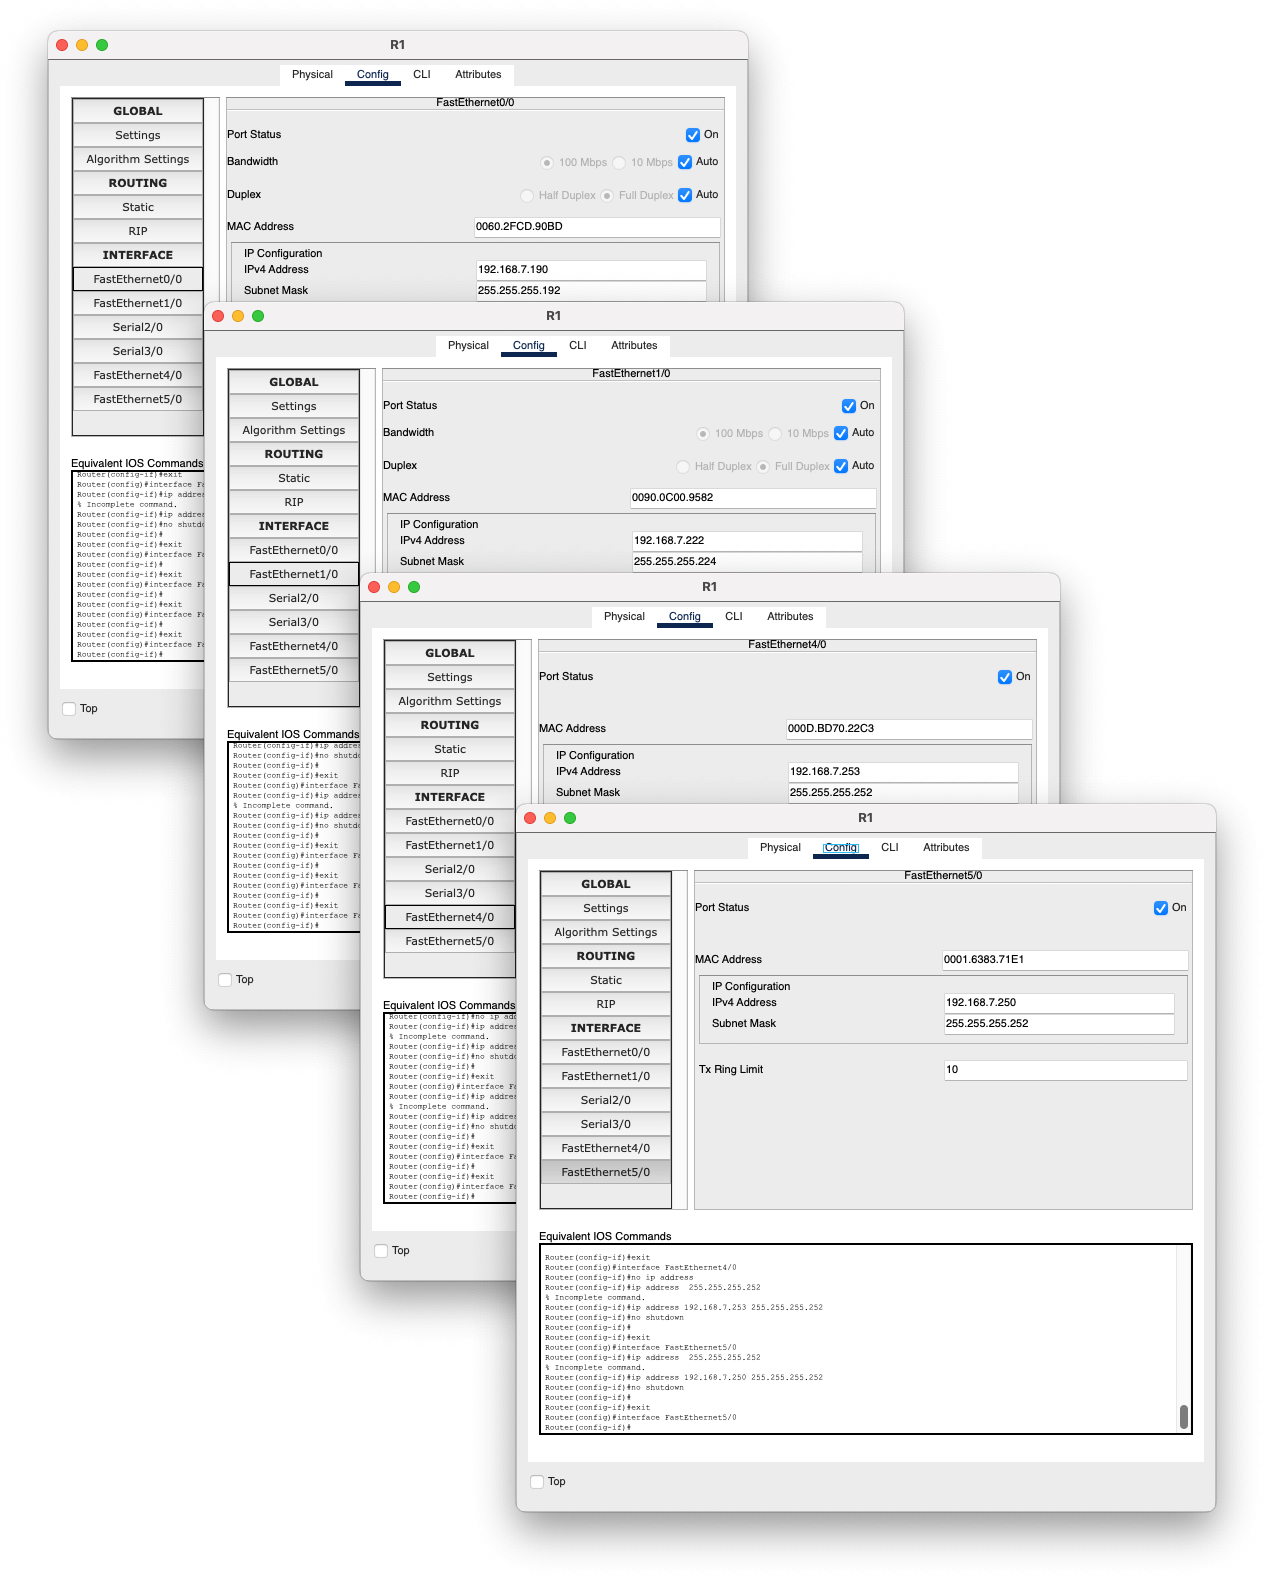
\includegraphics[scale=0.22  ,valign=c]{r1-ipall}                      \\ \hline
                        IP configuration for Router 2.  & 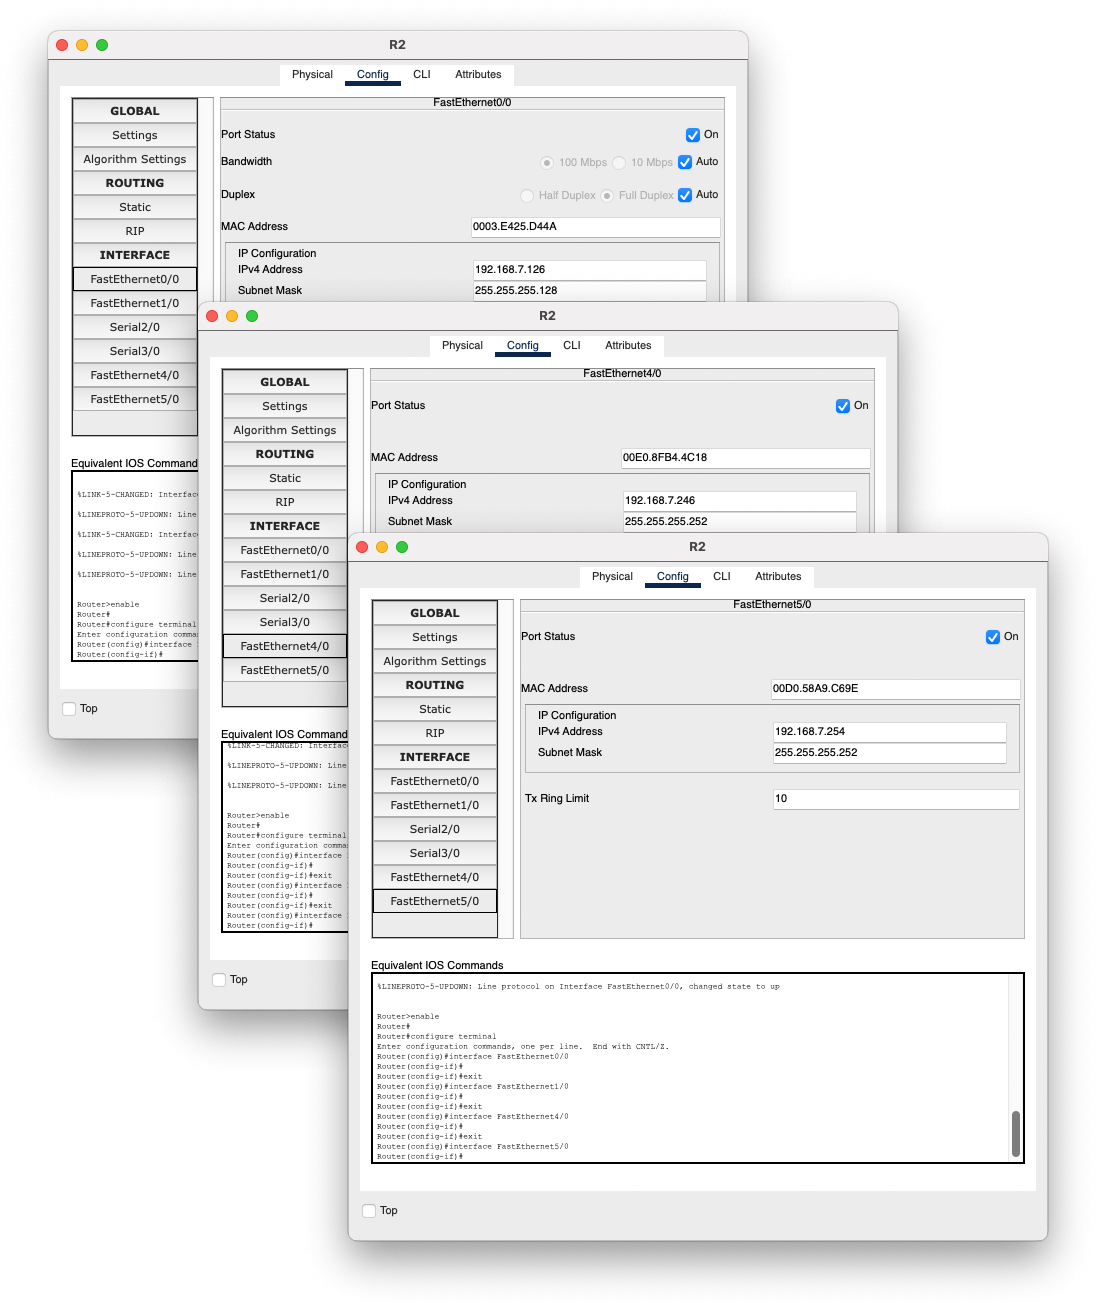
\includegraphics[scale=0.245 ,valign=c]{r2-ipall}                      \\ \hline
                        Static routes for Router 0.     & 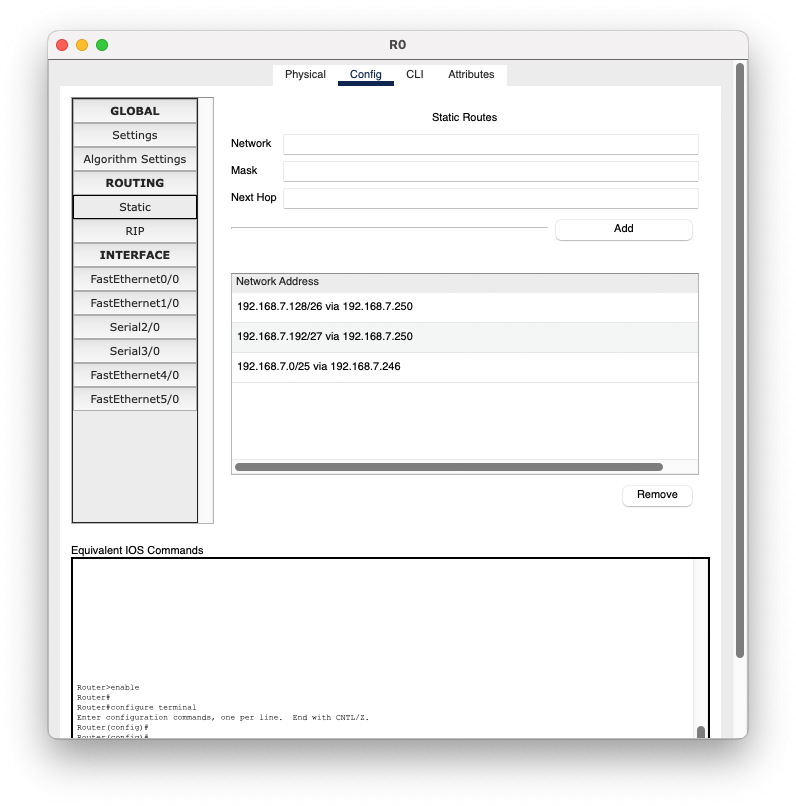
\includegraphics[scale=0.35  ,valign=c]{r0-staticroute}                \\ \hline
                        Static routes for Router 1.     & 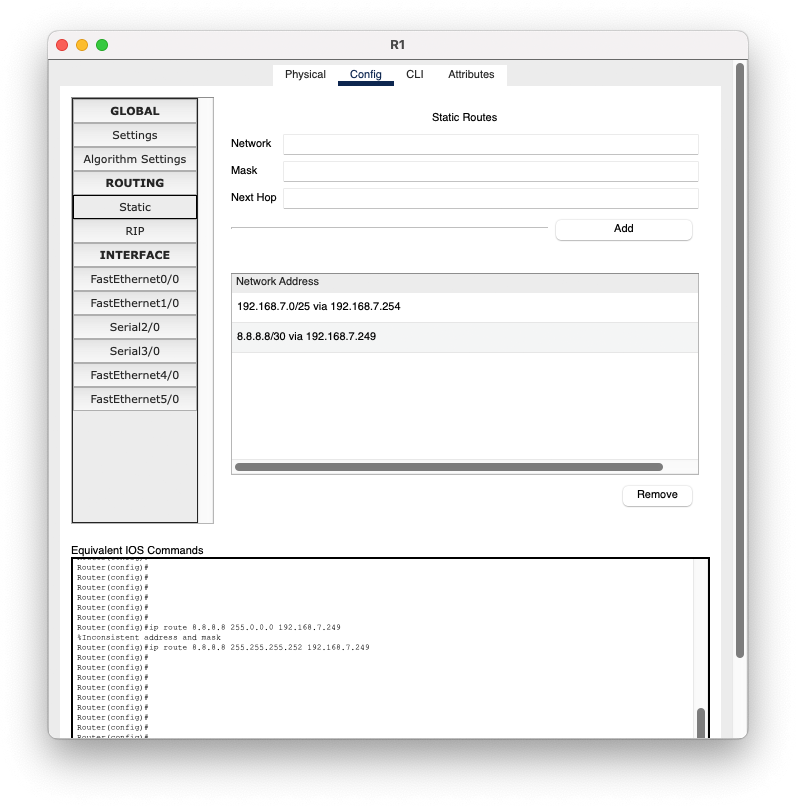
\includegraphics[scale=0.35  ,valign=c]{r1-staticroute}                \\ \hline
                        Static routes for Router 2.     & 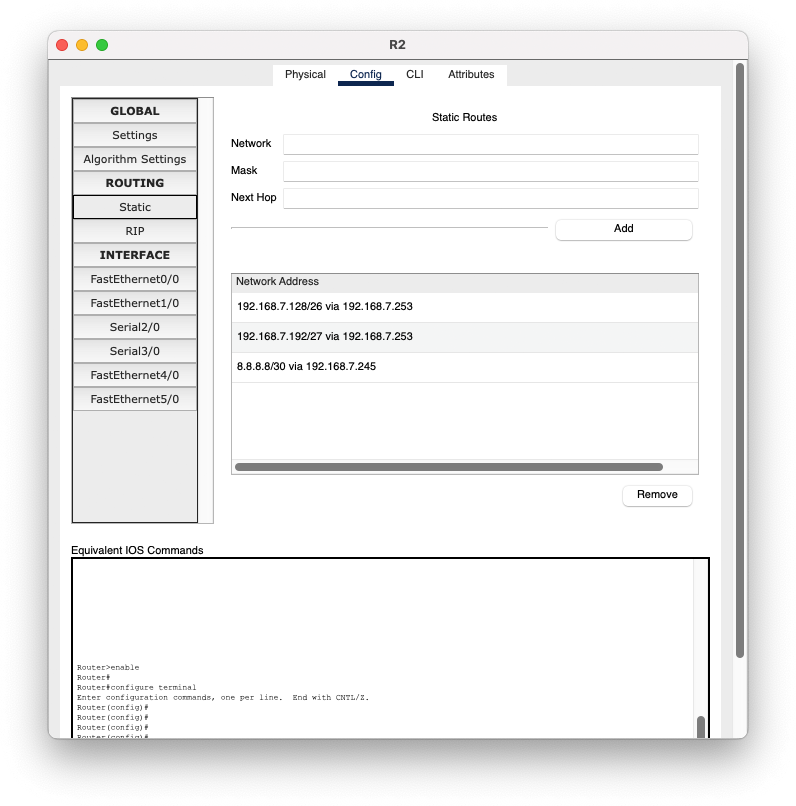
\includegraphics[scale=0.35  ,valign=c]{r2-staticroute}                \\ \hline

                        \caption{Cisco Packet Tracer IP router guide}
                        \label{tab:cptg1.5}
                    \end{longtable}
                \end{center}
        \end{flushleft}

    \section{Testing connectivity}
        After applying the configuration, we must test our network by running diagnostic commands. First arp, then ping, then arp again and finally tracert\footnote{Excluding commands to the device itself.}:

        \begin{longtable}[c]{@{}lll@{}}
            \toprule
            \textbf{Ping}      & \textbf{Trace Route}  & \textbf{Device} \\* \midrule
            \endfirsthead
            %
            \multicolumn{3}{c}%
            {{\bfseries Table \thetable\ continued from previous page}} \\
            \toprule
            \textbf{Ping}      & \textbf{Trace Route}  & \textbf{Device} \\* \midrule
            \endhead
            %
            \bottomrule
            \endfoot
            %
            \endlastfoot
            %
            arp -a             & arp -a                & ARP Table       \\
            ping 192.168.7.129 & tracert 192.168.7.129 & PC0             \\
            ping 192.168.7.130 & tracert 192.168.7.130 & Laptop0         \\
            ping 192.168.7.193 & tracert 192.168.7.193 & PC1             \\
            ping 192.168.7.194 & tracert 192.168.7.194 & Laptop1         \\
            ping 192.168.7.1   & tracert 192.168.7.1   & DHCP-Server     \\
            ping 192.168.7.2   & tracert 192.168.7.2   & DNS-Server      \\
            ping 192.168.7.3   & tracert 192.168.7.3   & HTTP-Server     \\
            ping 8.8.8.8       & tracert 8.8.8.8       & R0              \\
            ping 192.168.7.245 & tracert 192.168.7.245 & R0              \\
            ping 192.168.7.249 & tracert 192.168.7.249 & R0              \\
            ping 192.168.7.190 & tracert 192.168.7.190 & R1              \\
            ping 192.168.7.222 & tracert 192.168.7.222 & R1              \\
            ping 192.168.7.253 & tracert 192.168.7.253 & R1              \\
            ping 192.168.7.250 & tracert 192.168.7.250 & R1              \\
            ping 192.168.7.126 & tracert 192.168.7.126 & R2              \\
            ping 192.168.7.246 & tracert 192.168.7.246 & R2              \\
            ping 192.168.7.254 & tracert 192.168.7.254 & R2              \\* \bottomrule
            \caption{CLI commands}
            \label{tab:clicommands}\\
        \end{longtable}

        Since not everything fit in the images, their respective outputs are in the outputs subsection attesting to what was performed.

        \begin{flushleft}
                \begin{center}
                    \begin{longtable}{ m{5cm} l }
                        \textbf{Steps} & \textbf{Example} \\
                        \hline
                        \endfirsthead
                        \multicolumn{2}{c}%
                        {{\bfseries Table \thetable\ continued from previous page}} \\
                        \textbf{Steps} & \textbf{Example} \\
                        \hline
                        \endhead
                        \hline Continued on next page \\
                        \endfoot
                        \endlastfoot

                        To test the connection from devices we select a device by \textbf{single-clicking} it (1), go to the \textit{desktop tab} (2) and select \textit{Command Prompt} (3).                                               & 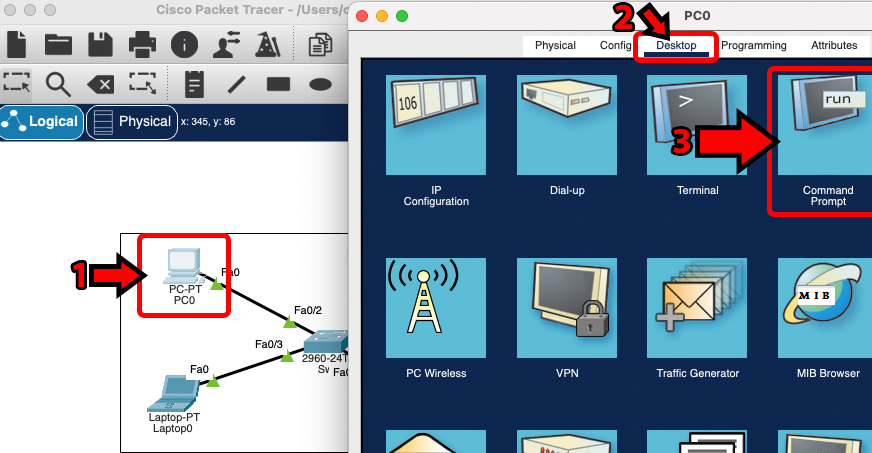
\includegraphics[scale=0.31 ,valign=c]{CiscoPacketTracer_cmdOutput}   \\ \hline
                        From LAN A, PC0 and Laptop0, viewpoint.                                                                                                                                                                             & 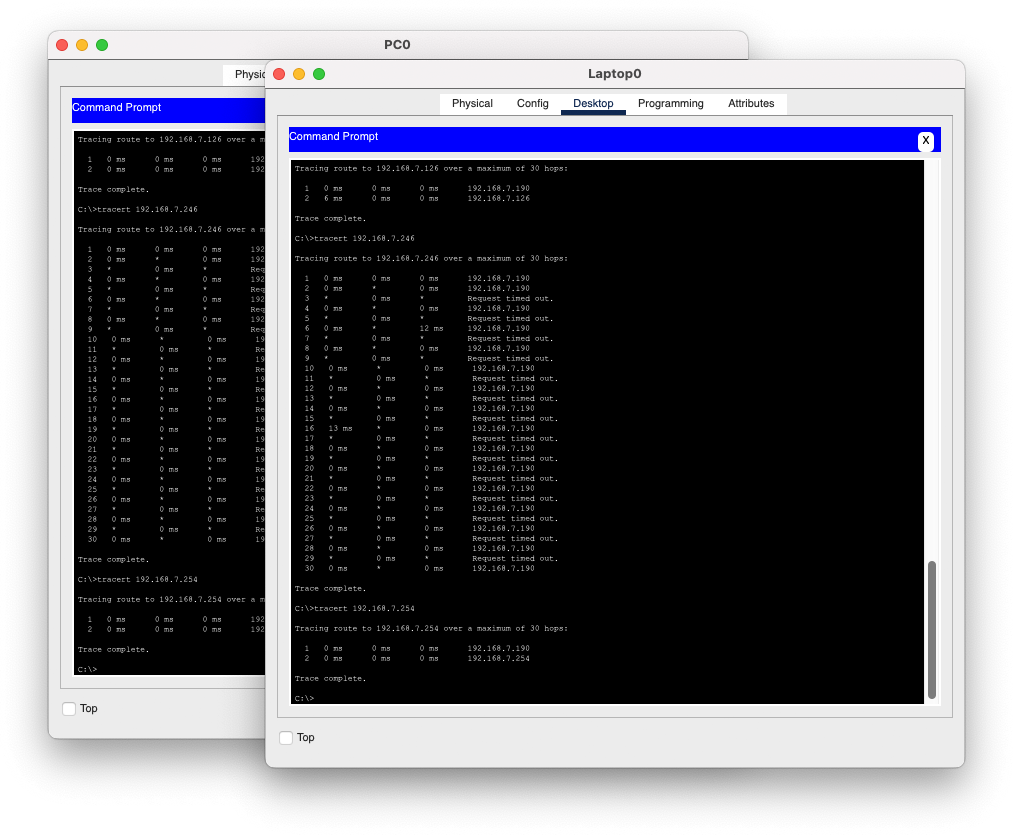
\includegraphics[scale=0.27 ,valign=c]{lana-outputall}                \\ \hline
                        From LAN B, PC1 and Laptop1, viewpoint.                                                                                                                                                                             & 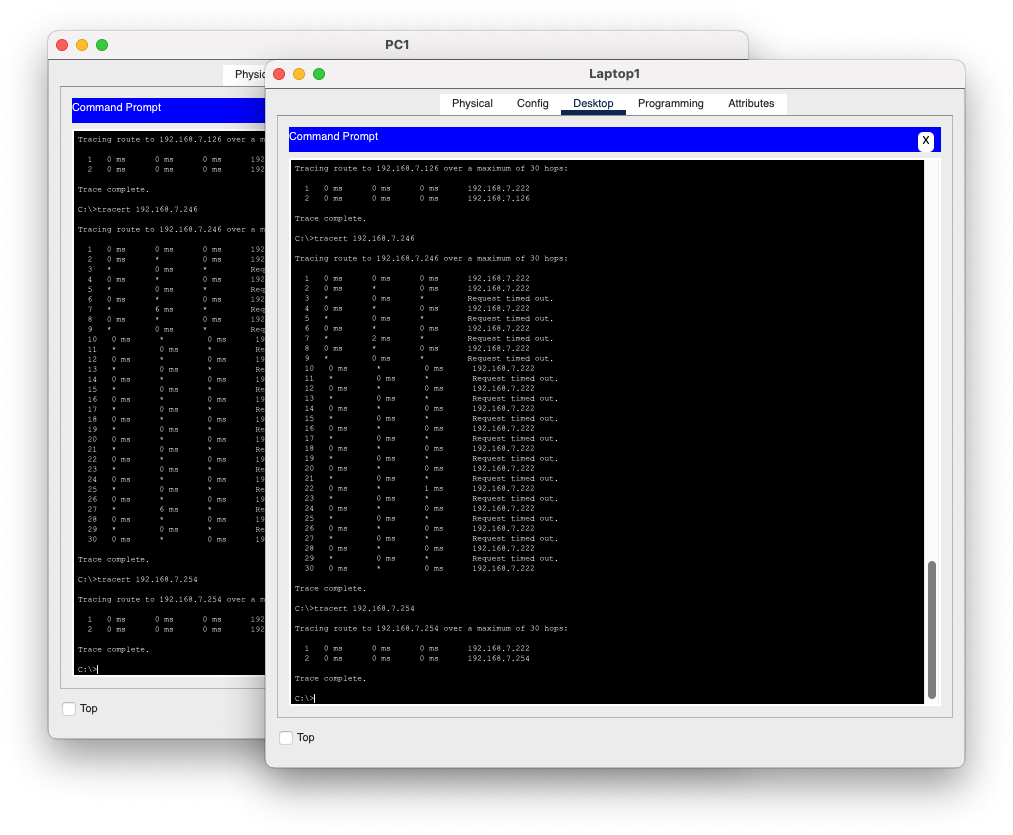
\includegraphics[scale=0.27 ,valign=c]{lanb-outputall}                \\ \hline
                        From LAN Servers, DHCP, DNS and HTTP servers, viewpoint.                                                                                                                                                            & 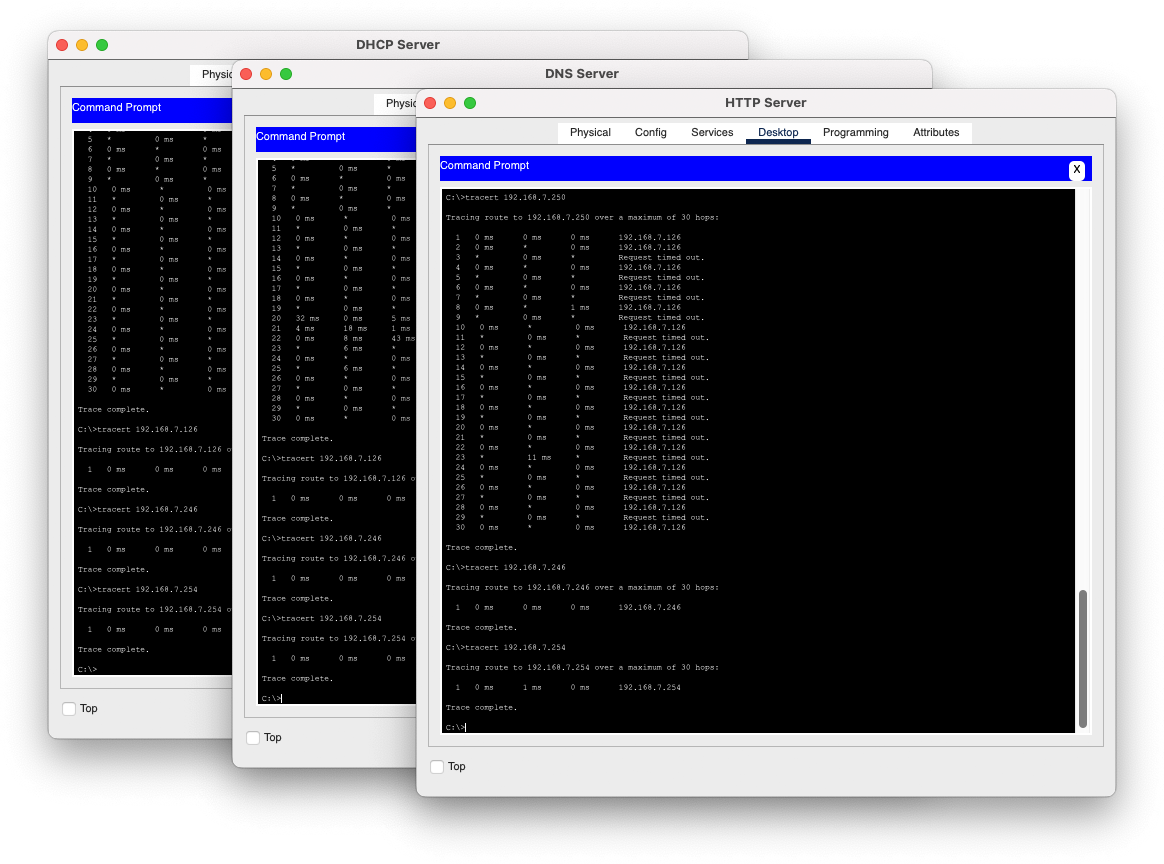
\includegraphics[scale=0.23 ,valign=c]{lanservers-outputall}          \\ \hline

                        \caption{Cisco Packet Tracer CLI device guide}
                        \label{tab:cptg2}
                    \end{longtable}
                \end{center}
        \end{flushleft}

        To test the connection from routers we select a router by \textbf{single-clicking}, go to the \textit{CLI tab}, input \textbf{exit} until \textbf{\textit{router>}} is shown, insted of \textbf{\textit{router\#}}.

        \begin{flushleft}
                \begin{center}
                    \begin{longtable}{ m{5cm} l }
                        \textbf{Steps} & \textbf{Example} \\
                        \hline
                        \endfirsthead
                        \multicolumn{2}{c}%
                        {{\bfseries Table \thetable\ continued from previous page}} \\
                        \textbf{Steps} & \textbf{Example} \\
                        \hline
                        \endhead
                        \hline Continued on next page \\
                        \endfoot
                        \endlastfoot

                        From router R0 viewpoint.   & 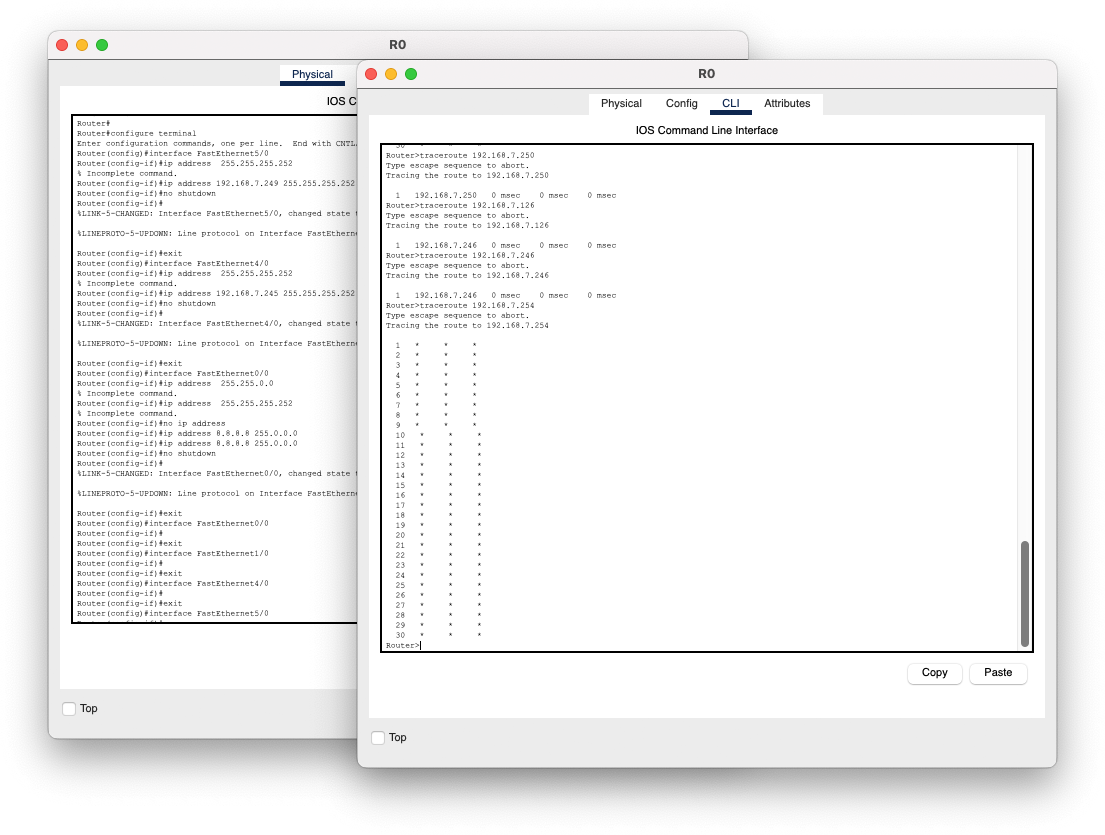
\includegraphics[scale=0.25 ,valign=c]{r0-cliall} \\ \hline
                        From router R1 viewpoint.   & 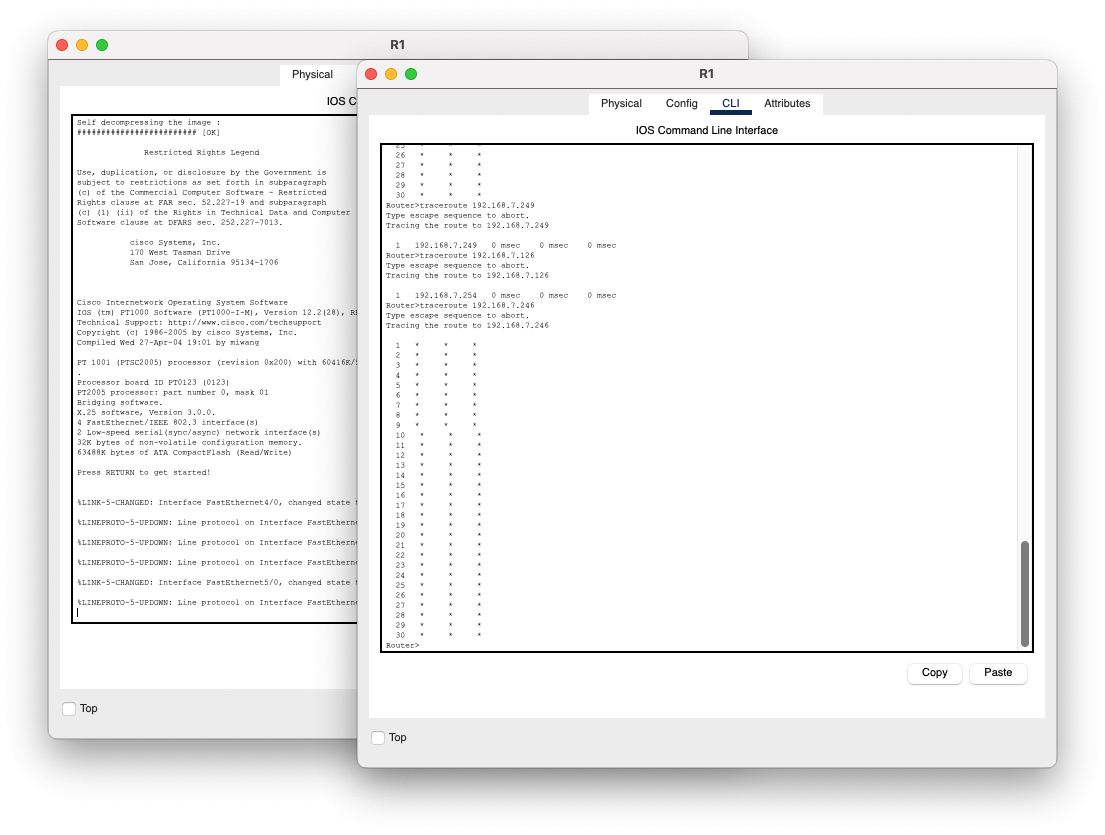
\includegraphics[scale=0.25 ,valign=c]{r1-cliall} \\ \hline
                        From router R2 viewpoint.   & 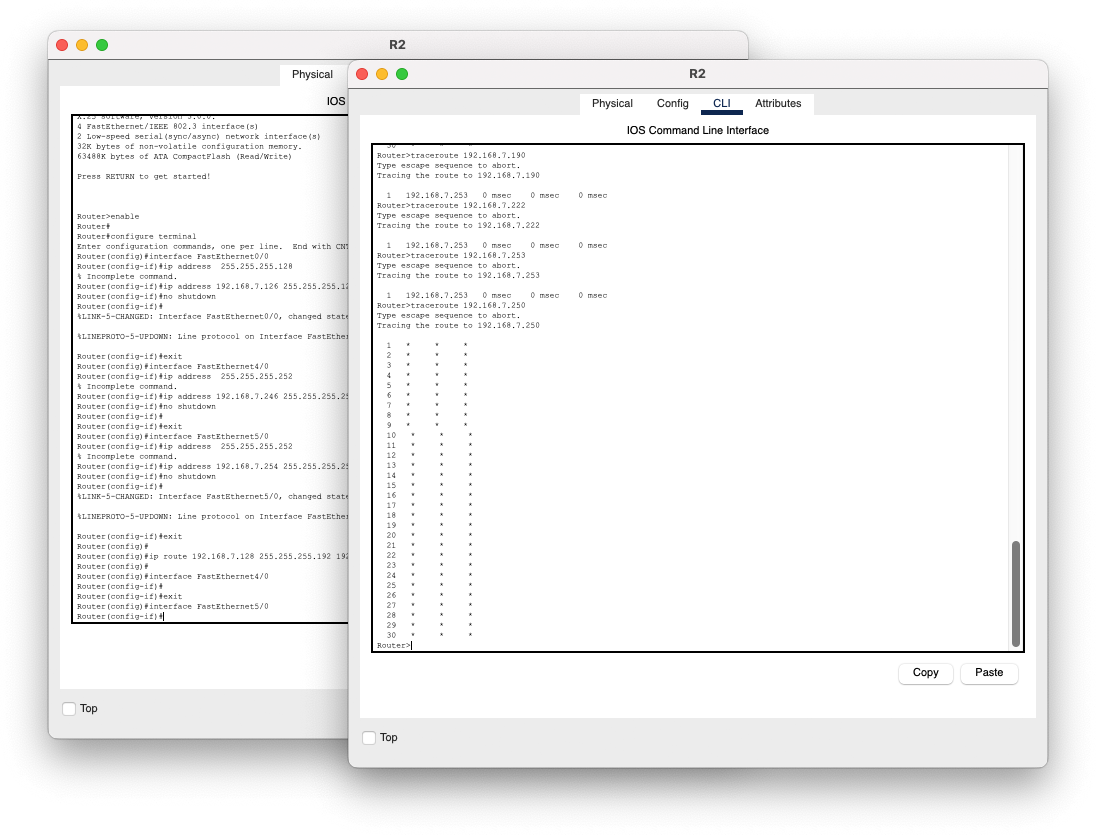
\includegraphics[scale=0.25 ,valign=c]{r2-cliall} \\ \hline

                        \caption{Cisco Packet Tracer CLI router guide}
                        \label{tab:cptg2.5}
                    \end{longtable}
                \end{center}
        \end{flushleft}

    \section{Command line outputs}
        To not over saturate the report, the outputs displayed only refer to one device per network. The others are in the \ref{clioutapxref} section from the appendix \ref{appendixref}.

        \lstset{style=termoutputs}
        \lstinputlisting[
            language={},
            caption={PC0 output (LAN A)},
            label={lst:pc0output}
        ]{./outputs/PC0.txt}

        \lstinputlisting[
            language={},
            caption={Laptop1 output (LAN B)},
            label={lst:laptop1output}
        ]{./outputs/Laptop1.txt}

        \lstinputlisting[
            language={},
            caption={DHCP-Server output (LAN Servers)},
            label={lst:dhcpoutput}
        ]{./outputs/DHCP-Server.txt}

        \lstinputlisting[
            language={},
            caption={Router 0 output},
            label={lst:r0output}
        ]{./outputs/R0.txt}

        \lstinputlisting[
            language={},
            caption={Router 1 output},
            label={lst:r1output}
        ]{./outputs/R1.txt}

        \lstinputlisting[
            language={},
            caption={Router 2 output},
            label={lst:r2output}
        ]{./outputs/R2.txt}

%% Chapter: issues and fixes ---------------------------------------------------
\chapter{Issues and fixes}
    \textbf{Cisco Packet Tracer in MacOS:}\\
        \hspace*{10mm}*STILL* no solution was found to deal with those annoying popups that takes primary focus over other windows, even using the latest version.\\
    \textbf{Misenterpretation of NATs:}\\
        \hspace*{10mm}Initially thought that static routes were meant to allow a certain network to go through another address. As it turned out it's quite the opposite, it should be understood as \textbf{\textit{I want to access LAN X from Router Y going through Router Z}}.

%% Chapter: conclusions --------------------------------------------------------
\chapter{Conclusions}
    We can actually see that everything complies with what was required.\\
    LAN A and B can only reach LAN Servers going through Router 1 and Router 2. They reach the outside through Router 1 and Router 0.\\
    LAN Servers reach LANs A and B through Router 2 and Router 1. External connections go over Router 2 and Router 0.\\
    This is possible because there isn't a static router designed to allow Router 1 to communicate with Router 0 with the intent to connect to LAN Servers.\\
    All of this is clear when reviewing the outputs. Most prominent with the \textit{Destination host unreachable} from ping and tracert's thirty retries outputing \textit{Request timed out} (or even the unmistakable hops taken when tracert is successful).

%% Bibliography ----------------------------------------------------------------
%\renewcommand{\bibname}{Bibliographic references}
%\bibliographystyle{chicago}
%\bibliography{refs}
%\addcontentsline{toc}{chapter}{\refname}  % add it to table of contents

%% Appendix --------------------------------------------------------------------
\appendix
    \chapter{Outputs}
    \label{appendixref}
        \section{Command line encore}
        \label{clioutapxref}

            \lstset{style=termoutputs}
            \lstinputlisting[
                language={},
                caption={Laptop0 output},
                label={lst:laptop0output}
            ]{./outputs/Laptop0.txt}

            \lstinputlisting[
                language={},
                caption={PC1 output},
                label={lst:pc1output}
            ]{./outputs/PC1.txt}

            \lstinputlisting[
                language={},
                caption={DNS-Server output},
                label={lst:dnsoutput}
            ]{./outputs/DNS-Server.txt}

            \lstinputlisting[
                language={},
                caption={HTTP-Server output},
                label={lst:httpoutput}
            ]{./outputs/HTTP-Server.txt}

\end{document}
